\documentclass[a4j, 11pt]{jreport}
% START:共通設定&共通パッケージ読み込み(基本変更しない)
\renewcommand{\baselinestretch}{1.4}
\setlength{\oddsidemargin}{-0mm}
\setlength{\textwidth}{16cm}
\setlength{\topmargin}{-1.5cm}
\setlength{\textheight}{24cm}
\setlength{\baselineskip}{2cm}
\special{pdf: minorversion=7}    % 出力するPDFのバージョンを指定
\usepackage{ifthen}              % if文制御用
\usepackage[dvipdfmx]{graphicx}
\usepackage{amsmath}             % 数式用
\usepackage{amsfonts}
\usepackage{array}               % 数式での場合分け用
\usepackage{url}                 % URL表示用
\usepackage{here}                % [H]用
\usepackage[dvipdfmx]{hyperref}  % 全体像把握&簡易移動のため
\usepackage{pxjahyper}           % 日本語のしおり(ブックマーク)表示用
\usepackage{bm}
\hypersetup{pdfborder = {0 0 0}} % hyperrefリンクの囲みを消す
\pagenumbering{roman}            % ページ番号をアラビア数字に変更
\newcounter{fiscal_year}         % 卒業年度計算用
\setcounter{fiscal_year}{\the\year}
\ifthenelse{\the\month < 4}{
	% 年明けから3月までは年-1にする
	\addtocounter{fiscal_year}{-1}
}{}
% END:共通設定&共通パッケージ読み込み(基本変更しない)


% START:ユーザ設定&ユーザパッケージ読み込み---------
\newcommand{\figref}[1]{\textbf{図~\ref{#1}}}
\newcommand{\tabref}[1]{\textbf{表~\ref{#1}}}
\newcommand{\eref}[1]{式(\ref{#1})}
\renewcommand{\bibname}{参考文献}
% END:ユーザ設定&ユーザパッケージ読み込み-----------


\begin{document}
% START:タイトル
\begin{titlepage}\Large ~
{\normalsize \the\value{fiscal_year} 年度卒業}
\vfill
\begin{center}

% START: 論文の種類-------------------------------
%{\Huge 修士論文}
{\Huge 卒業論文}
% END: 論文の種類---------------------------------
\end{center}
\begin{center}

% START: 日本語タイトル---------------------------
深層学習を用いたロバストな白線補完
% END: 日本語タイトル-----------------------------
\end{center}
\begin{center}

% START: 英語タイトル-----------------------------
English Title
% END: 英語タイトル-------------------------------
\end{center}
\vfill
\begin{center}
\begin{tabular}{|c|l|}
\hline

% START: 論文の種類-------------------------------
%所属 & 新潟大学自然科学研究科 電気情報工学専攻・林隆史研究室 \\
所属 & 新潟大学工学部情報工学科・林隆史研究室 \\
% END: 論文の種類---------------------------------
\hline

% START: 在籍番号---------------------------------
在籍番号 & T16I273C \\
% END: 在籍番号-----------------------------------
\hline

% START: 論文著者---------------------------------
氏名 & 小松 耀人 \\
% START: 論文著者---------------------------------
\hline
\end{tabular}
\end{center}
\vspace{1cm}
\vfill
\end{titlepage}
\pagebreak
\addtocounter{page}{1}
\thispagestyle{empty}  % このページにページ番号を振らない
% END:タイトル

% START:アブストラクト-----------------------------
\section*{概要}
 近年高齢者による事故が増え自動運転への期待も高まっている.しかしながら現在の研究で最も高い精度を出している自動運転技術は高精度地図を必要とし,高精度地図が整備されている道路は先進国全体でも1\%に満たない.高精度地図を全道路に整備するのは作成に人の手を介する点や,一般道路は更新頻度も高いという点で非現実的である. ゆえに,出発地から目的地まで人の手を一切介さない完全な自動運転の実現には高精度地図に依存せず,自車の周りの状況を把握し,その情報をもとに適切な進路をリアルタイムに選択することが不可欠である.特に路面上の情報を画像などから計測し,自車が走行すべき車線を計算することは、乗車している人の安全を保証する意味で非常に重要である.しかし,一般道路には白線が途切れていたりかすれていたりする場所が散見され,現在の技術では線がない部分の認識はできず,それらが道路状況を把握することの障害となっている. そこで本研究では敵対的生成ネットワーク(GAN)を用いて,白線の途切れやかすれを自動補完する手法を提案する.
\section*{Abstract}
English Abstract Here

% END:アブストラクト-------------------------------

% START:目次作成
\newpage
\tableofcontents       % 目次作成
\thispagestyle{empty}  % このページにページ番号を振らない
\pagebreak
\pagenumbering{arabic} % ページ番号をアラビア数字に変更
% END:目次作成


% START:本編--------------------------------------
\chapter{はじめに}
近年高齢者による事故が増えているが、地方では車がないと生活が困難な地域もあり免許を返納してもらうことが非現実的な地域も多くある。また、健常者が移動手段として使う車でも事故のリスクを少しでも減らし安全な社会を実現すべく運転支援技術の高度化や出発地から目的地まで一切人の手を介することのない完全な自動運転の実現が急がれている。\\
\indent 現在の研究で最も完全な自動運転に近い運転支援を実現しているのは通常のカーナビゲーションシステムに使用されている2Dの俯瞰図ではなく、数センチメートル以内の誤差しかない超高精度の3D地図にさらに道路上の構造物、車線情報、路面情報などの「静的情報」、道路工事やイベントなどによる交通規制などの「準静的情報」、信号の現示情報などの「動的情報」、観測時点の渋滞状況などの「準動的情報」などを付加したものでこの地図が整備されているのは先進国全体で1\%未満である。このような地図の整備状況が未だに狭い理由としては、そもそもの作成に人力でCADを用いた細かい調整が必要なことに加え、一般道路は更新の頻度も高く新しい道路がどんどんと増えていくことや地点ごとの車線や路面の整備状況の差異が非常に大きく手動で逐一更新していくのは非現実的である。様々な機関が自動的に高精度地図を整備する技術を提案しているが、未だに一般道路を自動的に高精度な地図に起こすまでには至っていない。\cite{tri-ad}\cite{autolab}\\
\indent このような背景から自車の周囲の車線や路面の情報を観測し、活用していくことが完全な自動運転の実現には必要不可欠である。また、仮に高精度地図が普及したとしても搭乗者の安全を守り正確な自動運転を行うために自車からの周辺観測は非常に重要である。\\
\indent 現在製品化している運転支援技術は先行車がいてかつ高速道路上で限られた速度帯でのみなど非常に限られた状況でしか作動せず、完全な自動運転には程遠い。限られた状況でしか作動しない原因の一つに一般道路は高速道路などの高規格幹線道路とは異なり道路整備の頻度も低く舗装や塗装の基準も異なるので場所によって白線や横断歩道などの路面上の情報が不完全になっているものも多くこれらを含む路面情報を認識するには前処理として本来必要であるのに欠落している情報を補完する必要がある。\cite{road_design}\\
\indent 以上の点を踏まえて本研究では深層学習を用いた画像補完技術を用いて本来必要であるのに白線が消えたりかすれたりしている部分を補完することを目的とする。画像補完にはGenerative Adversarial Network(GAN)を用い、ニューラルネットワークを用いて白線があるべき領域を重点的に学習し、補完を試みる。\\
\indent 各章の説明(あとから)

\chapter{ニューラルネットを用いた機械学習}
本章では機械学習の中の一つであるニューラルネットについて基本的なことから説明し,次にCNN,GANの仕組みについて詳しく説明する.

\section{深層学習}
 深層学習は,\figref{fig:neuron}に示すような生物の脳の神経細胞をモデル化したニューロンを基にして,\figref{fig:tasou}のようにニューロンを多層に結合したモデル(ニューラルネットワーク)を用いる学習法である.個々のニューロン間の結合には重み$\bm{w}$というパラメータが与えられており,$\bm{w}$が更新されていく(学習する)ことで,問題にあった最適解を導く.この重み$\bm{w}$の学習法として,誤差逆伝播法を用いる.誤差逆伝播法は教師信号値$\bm{t}$と出力結果値$\bm{h(x)}$の誤差の大きさを表す損失関数$E$を定義し,$E$に対し各層の$\bm{w}$の微分係数(勾配)を求めることで$\bm{w}$を更新していく.\\
\begin{figure}[htbp]
	\begin{minipage}{0.5\hsize}
		\begin{center}
			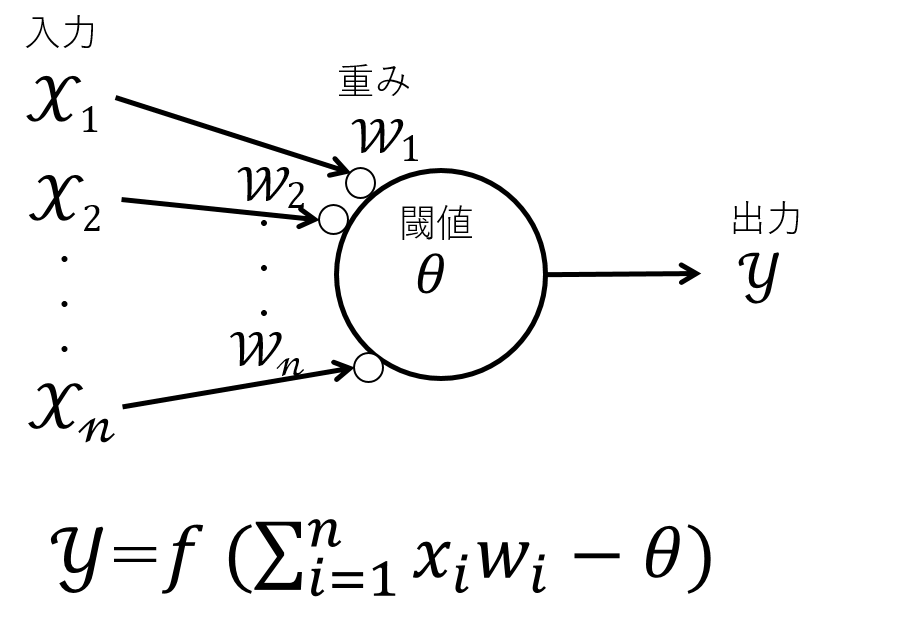
\includegraphics[scale=0.5]{./images/deeplearning/neuron_model.png}
			\caption{ニューロンモデル \label{fig:neuron}}
			
		\end{center}
	\end{minipage}
	\begin{minipage}{0.5\hsize}
		\begin{center}
			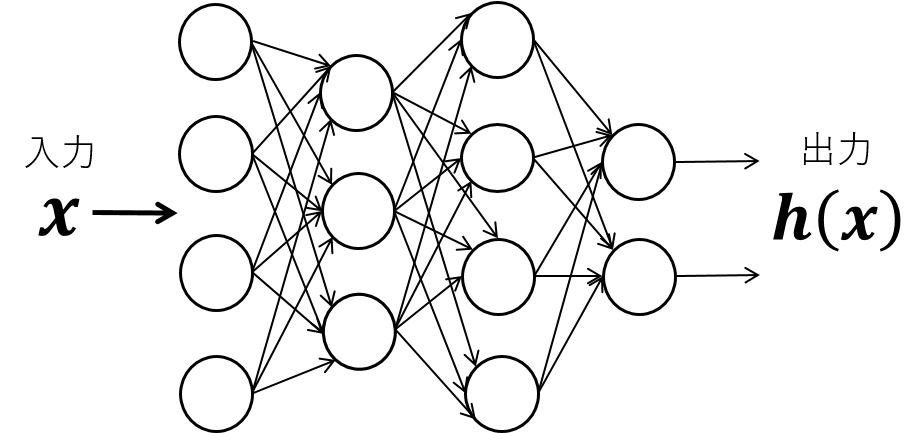
\includegraphics[scale=0.5]{./images/deeplearning/tasou.png}
			\caption{多層パーセプトロン \label{fig:tasou}}
			
		\end{center}
	\end{minipage}
\end{figure}

\section{損失関数と重み最適化}
\subsection{損失関数}
 損失関数$E$は様々な種類があり,一般的によく使われるものとして\eref{eq:loss-crossentropy}~\eref{eq:loss-abs}の,交差エントロピー誤差,平均2乗誤差,平均絶対誤差などがある.
 \begin{eqnarray}
	E &=& -\sum_{k}^{n} t_k log(h_{k}(\bm x)) \label{eq:loss-crossentropy} \\
	E &=& \frac{1}{n}\sum_{k}^{n}{( t_k - h_{k}(\bm x) )^2} \\
	E &=& \frac{1}{n}\sum_{k}^{n}| t_k - h_{k}(\bm x) | \label{eq:loss-abs}
\end{eqnarray}

\subsection{重み最適化}
$\bm{w}$を更新する手法は様々あるが,基本となっているものは\eref{eq:w_new}の勾配降下法であり,損失関数の勾配が減少する方向に学習率$\eta$を乗算した値を加えていくことで$\bm{w}$の最適値を見つけていく.
\begin{eqnarray}
	\label{eq:w_new}
	\bm{w_{t+1}} = \bm{w_{t}} - \eta \frac{\partial E}{\partial \bm{w}}
\end{eqnarray}
\begin{figure}[htbp]
	\begin{center}
		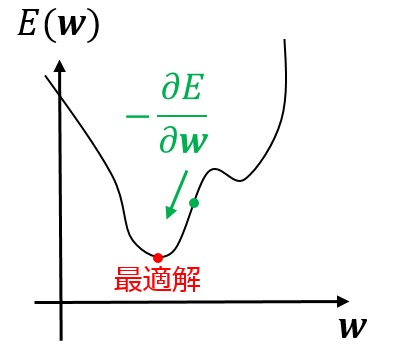
\includegraphics[scale=1]{./images/deeplearning/sgd.png}
		\caption{勾配降下法}
		\label{fig:sgd}
	\end{center}
\end{figure}

\newpage
\subsection{Adam}
Adamは\eref{eq:w_new}を派生させた$\bm w$の更新方法で現在よく用いられている最適化アルゴリズムである\cite{Adam}.
2015年にDiedeik P. Kingmaらが提唱した手法であり,\eref{eq:Adam}のように学習ステップごとに過去の勾配の値から勾配の重みつき平均と重みつき分散を推定している.これにより,更新が多い重みの学習率を低く,更新が少ない重みの学習率を高くするように設定され,学習の収束が早くなることが期待できる.\eref{eq:beta1}, \eref{eq:beta2}における$\beta_1,\beta_2$はハイパーパラメータを表し,実装する側が指定する値である.

\begin{align}
	\label{eq:Adam}
	\bm{w_{t+1}} &= \bm{w_{t}} - \eta \frac{\bm{\hat{m}}} {\sqrt{\bm{\hat{v}}} + \epsilon}\\
	\bm{\hat{m}} &= \frac{\bm{m_{t+1}}}{1-\beta_1^t} \nonumber \\
	\bm{\hat{v}} &= \frac{\bm{m_{t+1}}}{1-\beta_2^t} \nonumber
\end{align}
\vspace{-2zh}
\begin{align}
	\bm{m_{t+1}} &= \beta_1\bm{m_t} + (1-\beta_1) \frac{\partial E}{\partial \bm{w_t}} = (1-\beta_1) \sum_{i=1}^{t} \beta_{1}^{t-i} \bm{m_i} \label{eq:beta1} \\
	\bm{v_{t+1}} &= \beta_2\bm{v_t} + (1-\beta_2) (\frac{\partial E}{\partial \bm{w_t}})^2 = (1-\beta_2) \sum_{i=1}^{t} \beta_{2}^{t-i} \bm{v_i} \label{eq:beta2}
\end{align}


\newpage
\section{畳み込みニューラルネットワーク}
畳み込みニューラルネットワーク(CNN : Convolutional Neural Network)は,人間の視覚野の神経細胞の二つの働きである「画像の濃淡パターンを検出する(特徴抽出)」,及び「物体の位置が変動しても同一の物体であるとみなす(位置ズレの考慮)」を組み合わせたものとなっており,画像分野において高い評価を持つニューラルネットワークとなっている\cite{CNN}.また,入力データのパターンをうまく学習できるという点で,画像だけでなくを様々な問題設定でCNNが広く用いられ,高い精度を出している.

\figref{fig:CNN}は画像分類問題を例にとったCNNのモデルを示している.入力画像は特徴抽出部で特徴が抽出され,その特徴をもとに識別部でパターン分類を行う.特徴抽出部では数層の畳み込み層とプーリング層から構成され,識別部は全結合層から構成されている.
\\
\\

\begin{figure}[htbp]
	\begin{center}
		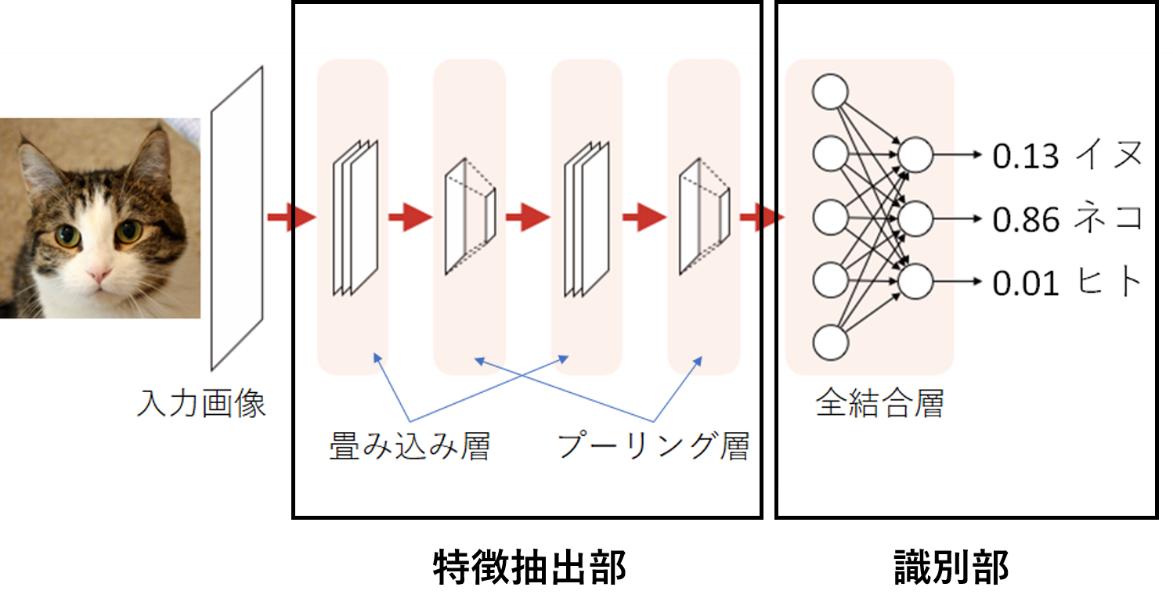
\includegraphics[scale=1.0]{./images/deeplearning/CNN.png}
		\caption{畳み込みニューラルネットワーク}
		\label{fig:CNN}
	\end{center}
\end{figure}

\newpage
\subsection{畳み込み層}
畳み込み層は画像の濃淡パターンを検出するための層に相当する.\figref{fig:convolution}に示すように,入力画像に対し各ピクセル値にフィルタを適用し,フィルタをスライドさせながら画像を圧縮し,特徴マップを作成する.学習時にはフィルタの値が更新される.
\begin{figure}[htbp]
	\begin{center}
		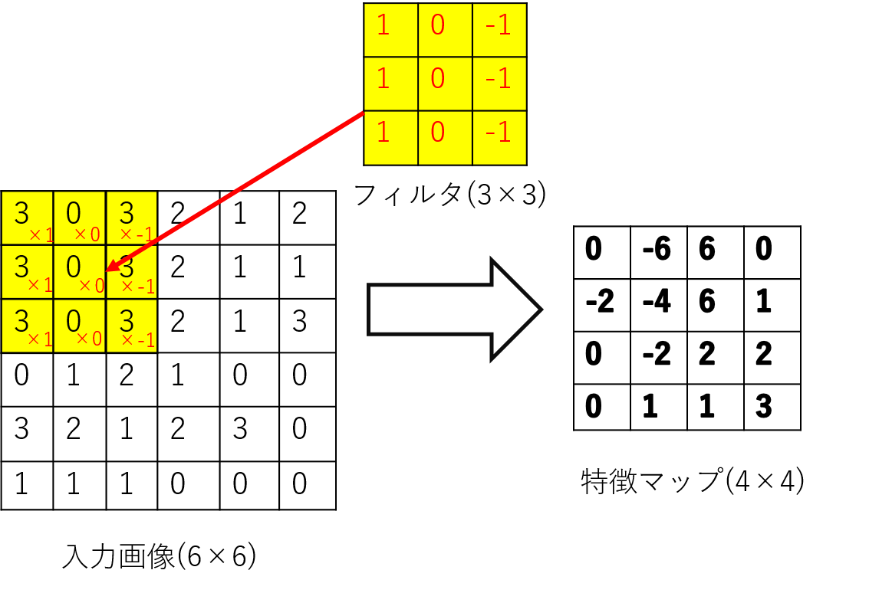
\includegraphics[scale=0.83]{./images/deeplearning/convolution.png}
		\caption{畳み込み}
		\label{fig:convolution}
	\end{center}
\end{figure}
\vspace{-40pt}
\subsection{プーリング層}
プーリング層は位置に対する感度を低くする代わりに,位置変化に対する認識能力を上げるための層に相当する.畳み込み層で得られた特徴マップに対しさらに圧縮をかけることで位置ズレの変化に対応する仕組みとなっている.圧縮のかけ方としては,最大プーリングと平均プーリングがある.\figref{fig:pooling}に示すのは最大プーリング(max pooling)であり,特徴マップの小領域の中から最大のピクセル値を得る操作となっている.対して平均プーリング(average pooling)は小領域の中の値を平均した値を得る操作となる.プーリング層においては学習時に更新されるパラメータは存在しない.

\begin{figure}[htbp]
	\begin{center}
		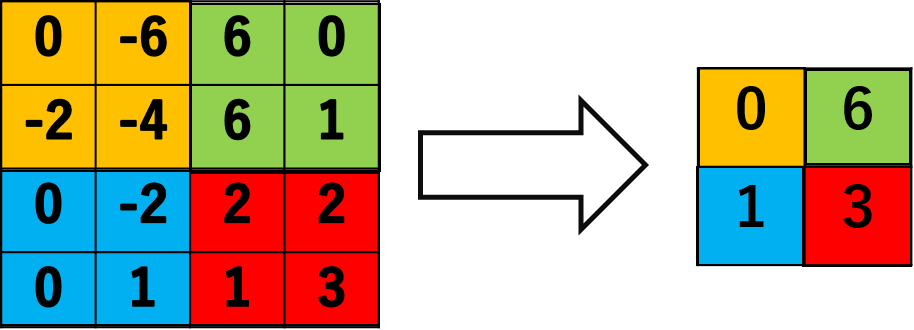
\includegraphics[scale=0.293]{./images/deeplearning/pooling.png}
		\caption{最大プーリング}
		\label{fig:pooling}
	\end{center}
\end{figure}

\newpage
\subsection{全結合層と活性化関数}
全結合層は,特徴抽出部から得られた特徴マップの値を入力とし,\figref{fig:tasou}のような多層パーセプトロンのニューラルネットワークによりパターン分類が行われる層である.最後のニューロンの出力数は問題設定に応じて変更される.分類問題の場合は分類したいクラス数であったり,画像生成問題の場合は画像のピクセルサイズ分の出力を持ったりなどをする.

各層のニューロンの出力値は活性化関数が通された後の値となっている.これは,ニューロンの出力が線形であるため,多層パーセプトロンと等価な1層のパーセプトロンの対が必ず存在してしまうことを避けるためである.活性化関数には,ランプ関数(ReLU),ソフトマックス関数,シグモイド関数などといったものが存在する.


\subsubsection{Relu関数}
中間層のニューロンの出力を非線形にするためによく使用されている関数である.非負の値を出力する.
\begin{eqnarray}
	f(x) = max(0, x)
\end{eqnarray}

\subsubsection{ソフトマックス関数}
ニューロンの出力を確率として扱う場合に使用される関数である.分類問題において最終層のニューロンの活性化関数として使用され,\eref{eq:softmax}で表される.
$a_k$は$k$番目のニューロンの出力値であり,$n$は最終層のニューロンの出力数である.
\begin{eqnarray}
	f_k(a_k) = \frac{e^{a_k}}{\displaystyle \sum_{i=1}^{n} e^{a_i}} \label{eq:softmax}
\end{eqnarray}

\subsubsection{シグモイド関数}
出力値を0~1に収める関数である.ニューロンの出力値を非線形したいときや,確率とみなしてマルチクラス分類をする際にも使用されている.
\begin{eqnarray}
	f(x) = \frac{1}{1+ e^{-x}}
\end{eqnarray}


\newpage
\section{敵対生成ネットワーク}
敵対生成ネットワーク(GAN : Generative Adversarial Network)は,学習データと似たような新しいデータを生成する生成モデルの一種であり,言い換えれば生成データの分布を学習データの分布に近づけていくように学習するモデルである.GANの構造を\figref{fig:GAN}に示す.GANは\figref{fig:GAN}に示すように,生成器(Generator)と識別器(Discriminator)から構成され,Generatorはランダムノイズからオリジナルと似たデータを生成し,Discriminatorは入力されるデータがGeneratorによって作られたデータか,それともオリジナルのデータかの識別を行う.これら二つのモデルが互いを見抜く・騙すように学習するため,十分に学習が進むとGeneratrはオリジナルのデータと見分けがつかないようなデータを生成するようになる.\\
\begin{figure}[htbp]
	\begin{center}
		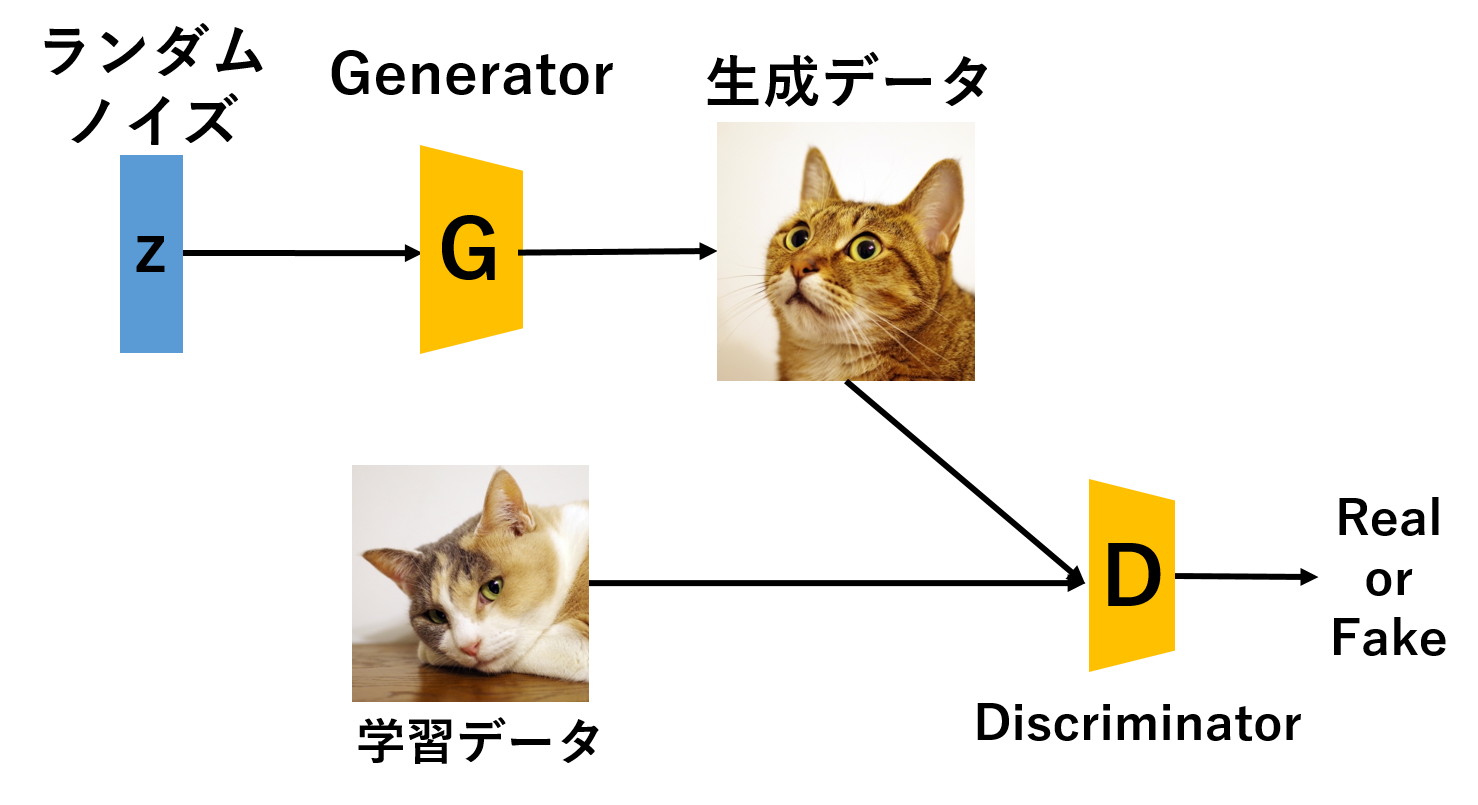
\includegraphics[scale=0.6]{./images/deeplearning/GAN.png}
		\caption{敵対生成ネットワーク(GAN)}
		\label{fig:GAN}
	\end{center}
\end{figure}

\newpage
\subsection{GANの損失関数}
具体的に評価関数を導入して学習を行う場合,\eref{eq:minimax}に関して,Discriminatorに対して最大化,Generatorに対して最小化するミニマックスゲームを考えればよい\cite{GAN}.
\begin{eqnarray}
	min_G max_DV(G, D) = \mathbb E_{\bm x \sim p_r(\bm x)}[{\rm log}D(\bm x)] + \mathbb E_{\bm z \sim p_z(\bm z)}[1 - {\rm log}D(G(\bm z))] \label{eq:minimax}
\end{eqnarray}
\eref{eq:minimax}において,$\bm x$はオリジナルデータ,$p_r(\bm x)$はオリジナルデータの確率分布,$\bm z$はランダムノイズ,$p_z(\bm z)$はランダムノイズの確率分布を示す.
この時,$D$がオリジナルのデータを正しく判定できれば${\rm log}D(\bm x)$が大きくなり,$D$が$G$の生成データをオリジナルのデータと誤って判定すると${\rm log}(1-D(G(\bm z)))$が小さくなる.

\subsection{GANの最適解}
\eref{eq:minimax}において,$\bm z \sim p_z(\bm z)$から$G$が生成するデータの分布を$p_g(\bm x)$とし,$V(G, D)$を書き直すと,
\begin{eqnarray}
	V(G, D) = \int_{\bm x} \{p_r(\bm x) {\rm log}D(\bm x) + p_g(\bm x) {\rm log}(1-D(\bm x)) \} \bm{dx}\label{eq:minmax}
\end{eqnarray}
となる.Discriminatorの最適解は$V(G, D)$を最大化することであるため,積分の中身の最大化をすればよい.よって中身を$D(\bm x)$に関して微分し,その時の導関数が0になる$D(\bm x)$を$D^*(\bm x)$とすると,\eref{eq:dis_opt}となる.
\begin{eqnarray}
	D^*(\bm x) = \frac{p_r(\bm x)}{p_r(\bm x) + p_g(\bm x)}\label{eq:dis_opt}
\end{eqnarray}
またこのとき,Generatorの最適化を考える.\eref{eq:dis_opt}の右辺を\eref{eq:minmax}に代入し式を整理すると,\eref{eq:jensengan}となる.
\begin{eqnarray}
	V(G, D) = 2D_{JS}(p_r||p_g)-\rm log4 \label{eq:jensengan}
\end{eqnarray}
\eref{eq:jensengan}を最小化することは,Jensen-Shannonダイバージェンスの最適化と等しく,$p_g = p_r$のときに最小値$- \rm log4$をとる.

\chapter{既存手法}
本章では、本研究に関連がある研究事例をあげ説明し、問題点となるところを考察する。
\section{VPGNet: Vanishing Point Guided Network for Lane and Road Marking
Detection and Recognition}
\subsection{}


% END:本編----------------------------------------

% START:参考文献----------------------------------
%% ベタ打ちの場合
\newpage
\begin{thebibliography}{1}
	\bibitem{tri-ad}TRI-AD\\ \url{https://www.tri-ad.global/jp/news/20190425} (2020年01月27日アクセス) 
	\bibitem{autolab}自動運転LAB\\ \url{https://jidounten-lab.com/u_autonomous-map-company} (2020年01月27日アクセス)
	\bibitem{road_design}第6章 道路舗装に関する設計基準\\ \url{http://www.mlit.go.jp/sogoseisaku/inter/keizai/gijyutu/pdf/road_design_j2.pdf} (2020年01月27日アクセス)
	\bibitem{Adam}
	Diederik P. Kingma, Jimmy Lei Ba, ”ADAM: A Method for Stochastic Optimizer, ”

	\bibitem{CNN}
	畳み込みニューラルネットワーク\\ \url{https://ml4a.github.io/ml4a/jp/convnets/}(2020年01月27日アクセス)

	\bibitem{GAN}
	”GANと損失関数の計算についてまとめた,” \\
	\url{https://qiita.com/kzkadc/items/f49718dc8aedbe8a1bee} (2020年01月27日アクセス)
	\bibitem{key1}サイト名\\ \url{http://google.com} (yyyy年mm月dd日アクセス)
	\bibitem{key1}サイト名\\ \url{http://google.com} (yyyy年mm月dd日アクセス) % ウェブサイトの場合
\bibitem{key2}著者,書籍タイトル,出版                                      % 書籍,論文の場合
\end{thebibliography}


%% bibtexを使用する場合
%\bibliography{ref}         % .bibファイルから拡張子を外した名前 ex)ref.bib
%\bibliographystyle{junsrt} % 参考文献出力スタイル
%\nocite{*}                 % 参照していない項目も出力する
% END:参考文献------------------------------------


\newpage
\section*{謝辞}
本研究を進めるにあたり,ご指導を頂いた林隆史教授に厚く感謝申し上げます.
また,日常の議論を通じて多くの知識や示唆を頂いた林隆史研究室の皆様に感謝いたします.

\end{document}
%------------------------------------------------
